\section{Klasyfikatory}

Przed przystąpieniem do przeprowadzenia pierwszych treningów pozostały do wykonania dwie czynności. Po pierwsze należało uzupełnić tworzony pakiet oprogramowania o~narzędzia umożliwiające wygodne konfigurowanie parametrów uczenia. Oparcie projektu także i~w~tym aspekcie o~pliki konfiguracyjne pozwoliło ostatecznie odseparować sferę wytwarzania modeli od detali implementacyjnych oraz ujednoliciło sposób organizacji pracy w~zespole. W~zaproponowanym rozwiązaniu wykorzystano dodatkowo mechanizm \textit{Tensorboard}, który umożliwia monitorowanie szerokiego zbioru statystyk w~trakcie treningu.

Ostatnim krokiem na drodze do rozpoczecia uczenia było ustalenie zestawu parametrów. Aby móc porównać skuteczność działania oraz efektywność uczenia w~przypadku różnych podejść opisanych w~projekcie przyjęto, że parametry te powinny być stałe na przestrzeni wszystkich treningów \footnote{W~ramach projektu przeprowadzono kilka pobocznych treningów modyfikujących przyjęte wartości parametrów, w~celu zbadania ich wpływu na proces uczenia.}. W~ten sposób przyjęto:

\begin{itemize}
    \item rozmiar porcji (ang. \textit{batch size}): 64
    \item initializacja wag i~obciążeń: inicjalizacja Glorota z~rozkładem normalnym
    \item algorytm optymalizacji: Adam
    \item funkcja strat: kategoryczna entropia skrośna
    \item krok uczenia (ang. \textit{learning rate}): adaptacyjny (początkowo $10^{-4}$)
\end{itemize}

Rozmiar porcji oraz optymalizator przyjęto na podstawie obserwacji doboru tych parametrów w~szeregu artykułów analizowanych w~ramach przygotowań do projektu. Sugerując się rozważaniami teoretycznymi oraz wynikami zaprezentowanymi w~pracy autorstwa X.~Glorota oraz Y.~Bengio \cite{glorot} zdecydowano się na wykorzystanie zaproponowanej przez nich metody inicjalizacji z~rozkładem normalny. Zapewnia ona zdaniem twórców odpowiednie zależności statystyczne pomiędzy parametrami kolejnych warstw sieci, co prowadzić ma do zmniejszenia ryzyka wystąpienia zjawisk zanikającego oraz eksplodującego gradientu. Przeprowadzona w~artykule analiza zakłada wykorzystanie nieliniowości typu sigmoidalnego. Niestety artykuł rozważający analogiczne rozwiązanie dla funkcji aktywacji typu ReLU (wykorzystanej w~projekcie) autorstwa Kaiminga He et al. \cite{he} został znaleziony przez zespół dopiero po wykonaniu serii treningów. Ze względu na zadowalające rezultaty zdecydowano nie powtarzać uczenia ze zmienioną metodą inicjalizacji.

Jako funkcję strat przyjęto początkowo kategoryczną entropię skrośną. W~późniejszym etapie zaczęto rozważać również funkcję Hinge'a. Bazując na rozważaniach teoretycznych \cite{rosasco} oraz analizie praktycznej \cite{janocha} zdecydowano się jednak pozostać przy pierwotnym wyborze. W~procesie uczenia wykorzystano adaptacyjną wielkość kroku. Jego wartość początkową ustalono na bazie pobieżnej analizy przypadków. Krok zmniejszany był \mbox{$0.02-$krotnie}, gdy wartość straty na zbiorze walidacyjnym nie malała na przestrzeni 4~epok. Tak obrana strategia pozwoliła znacząco zwiększyć efektywność treningów.

\vspace{0.5cm}
\begin{figure}[h]
    \centering
    \begin{subfigure}{.5\textwidth}
        \centering
        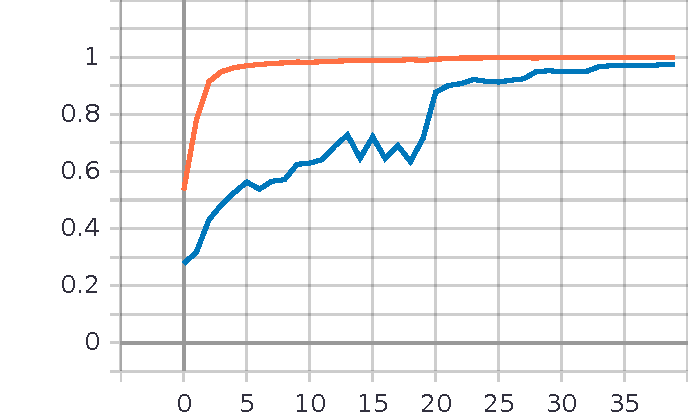
\includegraphics[scale=0.6]{img/adaptive_lr_accuracy.pdf}
      \end{subfigure}%
      \begin{subfigure}{.5\textwidth}
        \centering
        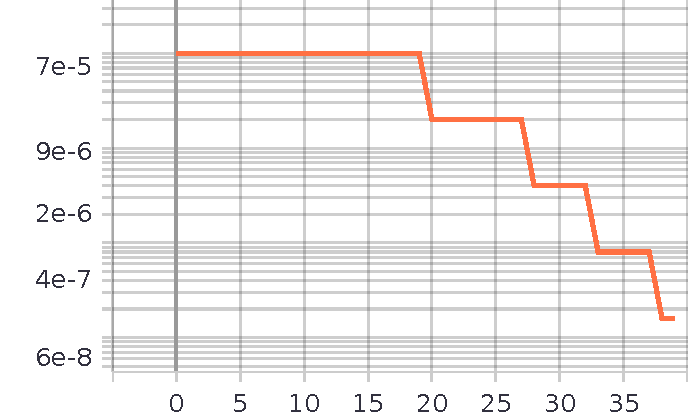
\includegraphics[scale=0.6]{img/adaptive_lr_lr.pdf}
      \end{subfigure}
      \captionsetup{format=plain,justification=centering}
      \caption{\small Przebieg dokładności modelu oraz wielkości kroku uczeni w~procesie uczenia (przypadek uczenia całej sieci).}
    \label{adaptive_lr_img}
\end{figure}
\vspace{0.5cm}

\subsection{Klasyfikator perceptronowy}

\subsection{Maszyna Wektorów Wspierających}

\subsection{Porównanie wyników}

